% !TEX root = ../manuscript.tex
\section{Method}
\label{sec:methods}

\subsection{Workflow Overview}

SC-FMA takes exposed process artifacts through sequence normalization, graph construction, SCU calibration, and audit-record emission.

The input is a set of observable knowledge artifacts such as retrieval checks, entity bindings, rule-like operations, verification records, or reflective annotations. These artifacts are normalized into an auditable sequence, converted into a graph representation with temporal and optional domain edges, calibrated by SCU against the supplied annotation or utility signal, and emitted as audit records. The empirical study evaluates this record behavior with representation readouts.

\subsection{SC-FMA as a Representation Layer}

SC-FMA represents structural dependencies among intermediate knowledge artifacts and converts them into audit-oriented records. The records preserve fidelity information while adding structural-role and interpretation fields.

\subsection{Formal Problem Definition}

SC-FMA takes an observable artifact sequence $T=(s_1,\ldots,s_k)$, where each unit $s_i$ may be a verification, reflection, retrieval, entity-binding, or rule-like operation available for audit. The sequence is converted into a graph $G=(V,E)$ whose nodes correspond to artifact units and whose edges encode temporal adjacency plus optional topical or domain-specific relations. The method also receives a utility or fidelity field $u$ over the same units. This field may come from local utility estimation, a proxy representation field, or a learned step-annotation model, and SC-FMA treats it as the fidelity field to be preserved when it is informative.

The output is a set of calibrated knowledge artifact records. Each record contains an audit-priority field plus fidelity, structural-dependency, redundancy, bottleneck, audit-reason, and interpretation fields. The objective is to preserve useful utility information, incorporate observable artifact structure, and attach each selected artifact to an interpretable audit-oriented analysis.

\subsection{SCU Objective and Audit Decomposition}
\label{sec:scu-objective}

SCU is a representation constraint system for fixed-budget audit records. It tracks an informative fidelity field when available while making the structural reason for each priority visible. Dependency, redundancy, and bottleneck fields indicate whether a selected artifact is local evidence, dependency support, repeated support, or a later-artifact dependency.

For an artifact sequence with $k$ auditable units, let $\tilde{\mathbf{c}}\in\mathbb{R}^k$ denote the normalized utility or proxy-fidelity field. In the locked PRM800K process-annotation stage, \wstruct{} denotes the output of the frozen Ridge regressor, used as this fidelity field. In the binary-correctness local-utility setting, $\tilde{\mathbf{c}}$ is a coarse sequence-level local utility anchor: it records how an observed outcome changes under a documented intervention. Let $\tilde{\mathbf{n}}$ denote normalized structural necessity from graph perturbation checks, $\mathbf{R}$ a redundancy matrix, and $\mathbf{b}$ a bottleneck indicator. The main notation is summarized in Table~\ref{tab:notation}.

\begin{table}[ht]
\caption{Notation used by the SCU objective and audit-record fields.}
\label{tab:notation}
\centering
\small
\renewcommand{\arraystretch}{1.08}
\begin{tabular}{Z{0.18\linewidth}Z{0.70\linewidth}}
\toprule
\textbf{Symbol} & \textbf{Meaning in this paper} \\
\midrule
$\tilde{\mathbf{c}}$ / \wstruct{} & Normalized fidelity field; in the locked PRM800K stage, \wstruct{} is the dev-trained frozen Ridge fidelity field. \\
$\tilde{\mathbf{n}}$ & Normalized structural-necessity field from graph perturbation checks. \\
$\mathbf{R}$ & Redundancy matrix over auditable artifact units. \\
$\mathbf{b}$ & Bottleneck indicator vector. \\
$\mathbf{w}$ & Calibrated audit-priority field on the probability simplex. \\
$\alpha,\beta,\gamma,\delta$ & Fidelity, structural-necessity, redundancy, and bottleneck coefficients in SCU. \\
Ridge / QP / Projection & Preservation softmax, constrained SCU solver, and topology-constrained simplex projection variants. \\
\bottomrule
\end{tabular}
\end{table}

SC-FMA computes calibrated priority-field values $\mathbf{w}$ on the probability simplex
\begin{equation}
\mathcal{W}=\{\mathbf{w}\in\mathbb{R}_{+}^{k}: \sum_i w_i = 1\}
\label{eq:scu-feasible-set}
\end{equation}
by minimizing the SCU objective:
\begin{equation}
L(\mathbf{w}) =
\alpha\|\mathbf{w} - \tilde{\mathbf{c}}\|_2^2
+ \beta\|\mathbf{w} - \tilde{\mathbf{n}}\|_2^2
+ \gamma\,\mathbf{w}^{\top}\mathbf{R}\mathbf{w}
- \delta\sum_i b_i \log(w_i).
\label{eq:scu}
\end{equation}
Unless otherwise stated, $\alpha,\beta,\gamma,\delta \ge 0$ and the symmetric part of $\mathbf{R}$ is treated as positive semidefinite on the simplex tangent subspace. The terms encode fidelity, structural alignment, redundancy regularization, and non-zero bottleneck regularization. The fidelity field is dominant; redundancy and bottleneck terms mainly encourage interpretable decomposition fields under the current validation setting. Detailed notation, construction rules, algorithms, and proofs are provided in the supplementary material.

\subsection{Artifact Representation}

Each artifact sequence is represented as an ordered set of auditable knowledge artifacts. The implementation supports units from structured reflection tags and free-text chain-of-thought segmentation, so segmentation is an observed pipeline input rather than a latent construct.

A node $v_i$ corresponds to one artifact unit. Temporal edges connect adjacent units, while topical edges connect units whose TF-IDF similarity exceeds the configured threshold. The graph serves as the representation substrate for knowledge dependencies. TF-IDF provides a lightweight fallback backend when richer domain relations are unavailable.

A supplementary graph-construction ablation replaces TF-IDF topical edges with Sentence-BERT embeddings (\texttt{sentence-transformers/all-MiniLM-L6-v2}, 384 dimensions). In that 800-trace fixture, the TF-IDF topical default (0.0515) did not exceed temporal-only edges (0.0596) on structural-necessity consistency. The embedding backend (0.0615) was only slightly higher on the same readout.

These differences are too small to treat topical edges as a representation-field driver. We therefore read the graph layer as an interchangeable \emph{construction interface}. In this setting, the TF-IDF topology adds little annotation-order preservation value over the temporal chain and functions mainly as a fallback lexical cue; if the structural field is used for ranking rather than audit-record construction, this weak and sometimes negative alignment is a material limitation.

The graph constructor is modular. Semantic embeddings, entity links, knowledge graphs, ontologies, rule-dependency DAGs, and data-lineage graphs can replace the default without modifying SCU. The Countries-KG study (Section~\ref{sec:kg-pilot}) and the embedding ablation illustrate this interface. We additionally implement a mathematical variable-dependency DAG that links a step to earlier steps introducing symbols that it references. This domain-motivated backend provides a direct graph-necessity control against the TF-IDF topology and a reverse-position baseline.

\subsection{Structural Necessity, Redundancy, and Bottlenecks}

Structural necessity measures how much graph support is lost when a node is perturbed under a documented graph-level operation. The implementation uses PRUNE, CASCADE, and BYPASS checks. PRUNE removes direct node support. CASCADE propagates disruption to downstream neighbors. BYPASS asks whether alternative paths can substitute for the removed artifact unit. The final necessity field $\tilde{\mathbf{n}}$ is the normalized summary of these observable graph checks.

The redundancy matrix $\mathbf{R}$ captures pairwise similarity between artifact units. High redundancy means that two units appear to serve overlapping functions. The penalty $\mathbf{w}^{\top}\mathbf{R}\mathbf{w}$ discourages allocating large budget share to many mutually redundant units. In the current evidence package, this term records duplicated-audit pressure, but its direct contribution to annotation-order consistency is modest.

Bottleneck detection addresses the opposite pattern. Some nodes are not redundant, and their downstream exposure can make them worth inspecting even if the supplied fidelity field is modest. The log-barrier prevents identified bottleneck nodes from receiving near-zero priority-field mass, keeping a possible single point of failure visible.

Figure~\ref{fig:local-utility-necessity} illustrates the local-utility--necessity mismatch. Figure~\ref{fig:variant-behavior} reports the three perturbation modes, and Figure~\ref{fig:resilience} shows the resilience curves. Together, the figures explain why the representation needs separate fidelity and structural fields: local utility, graph necessity, and resilience under removal capture related but distinct readouts.

\begin{figure}[pos=ht]
\centering
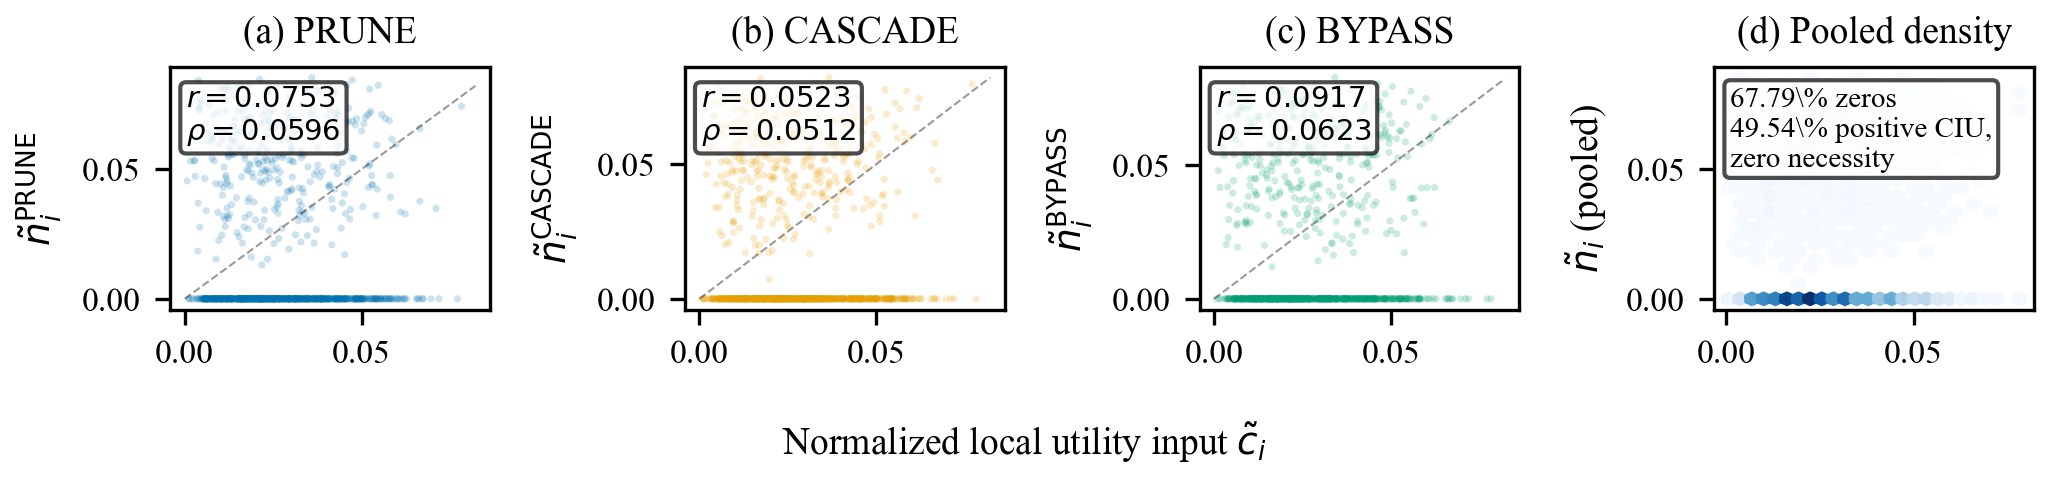
\includegraphics[width=\linewidth]{figures/fig_local_utility_necessity.png}
\caption{Structural mismatch motivating calibration. Local utility and graph-level necessity diverge: many locally useful steps have low measured structural necessity, while some structurally exposed steps receive limited local utility support. The shared $x$-axis $\tilde{c}_i$ denotes the normalized local utility field for step $i$. SC-FMA uses this mismatch as the reason for calibration.}
\label{fig:local-utility-necessity}
\end{figure}

\begin{figure}[pos=ht]
\centering
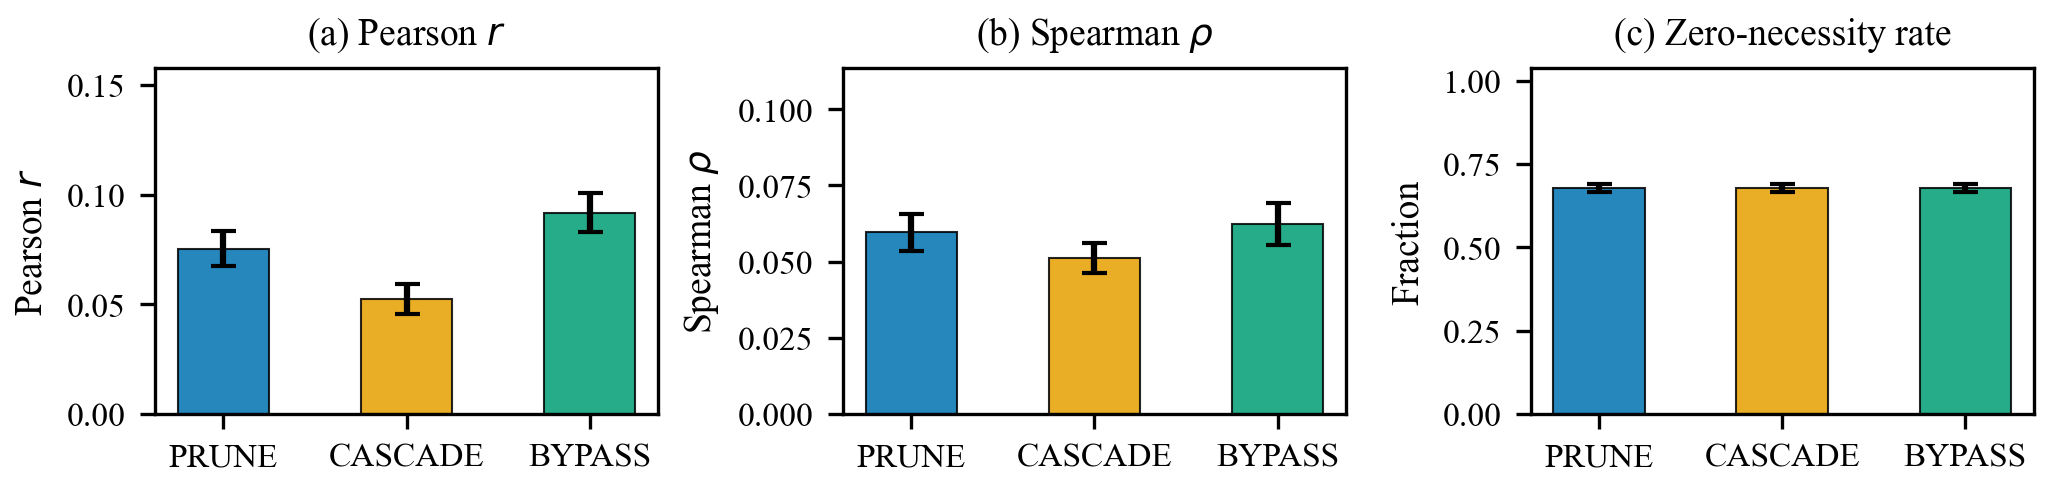
\includegraphics[width=\linewidth]{figures/fig_representation_variant_behavior.png}
\caption{Structural perturbation summary by mode. The three perturbation modes (PRUNE, CASCADE, BYPASS) are reported with Pearson correlation, Spearman annotation-order consistency, and zero-necessity fraction. Error bars indicate 95\% bootstrap confidence intervals. The consistency across modes indicates that weak local-utility--necessity alignment persists across perturbation strategies.}
\label{fig:variant-behavior}
\end{figure}

Figure~\ref{fig:variant-behavior} keeps the perturbation evidence at the representation-analysis level. PRUNE, CASCADE, and BYPASS expose how structural necessity is measured under different graph operations; their role is to test whether the mismatch is stable enough to justify a separate structural field. The low and negative correlations also bound the reading of this field: on lightweight lexical graphs for mathematical process annotations, structural necessity can be topology-sensitive or misaligned with human step labels and should be interpreted through graph-backend and perturbation checks rather than as an independent quality metric.

\begin{theorem}[SCU well-posedness]
\label{thm:scu-well-posedness}
Let $\mathbf{R}_{s}=(\mathbf{R}+\mathbf{R}^{\top})/2$ and let $\mathcal{T}=\{\mathbf{z}\in\mathbb{R}^{k}:\mathbf{1}^{\top}\mathbf{z}=0\}$ be the tangent subspace of the simplex. Define the quadratic Hessian on this subspace as $\mathbf{H}_{q}=2((\alpha+\beta)\mathbf{I}+\gamma\mathbf{R}_{s})$. Assume $\alpha,\beta,\gamma,\delta \ge 0$ and $\mathbf{z}^{\top}\mathbf{R}_{s}\mathbf{z}\ge 0$ for every $\mathbf{z}\in\mathcal{T}$. Then the SCU objective in Eq.~\ref{eq:scu} is convex on the relative interior of the simplex in Eq.~\ref{eq:scu-feasible-set}. If $\mathbf{z}^{\top}\mathbf{H}_{q}\mathbf{z}>0$ for every nonzero $\mathbf{z}\in\mathcal{T}$, the quadratic part is strictly convex on the feasible subspace and the minimizer is unique. If $\delta>0$ and $b_i=1$, any finite minimizer assigns $w_i>0$ to that bottleneck node; the barrier therefore gives an interior guarantee for active bottleneck support. For non-redundant artifact-unit pairs with identical redundancy profiles and inputs ordered in the same direction, $\tilde c_i\ge \tilde c_j$ and $\tilde n_i\ge \tilde n_j$, the two-input priority-field relation is monotone before redundancy-induced redistribution. Once redundancy profiles differ, this monotonicity remains a local interpretive property.
\end{theorem}

The theorem is a well-posedness check for the constrained representation program, not a source of empirical validation. Its monotonicity statement applies before redundancy-induced redistribution under matched redundancy profiles; the empirical sections therefore determine when the optimizer is useful or brittle.

We implement three variants of the same calibration procedure; they are not competing claims that one optimizer is universally best. SC-FMA Ridge uses a closed-form softmax over a linear combination of $\tilde{\mathbf{c}}$ and $\tilde{\mathbf{n}}$ and does not contain the $\gamma\mathbf{w}^{\top}\mathbf{R}\mathbf{w}$ redundancy term or the bottleneck log-barrier term. SC-FMA QP solves the full constrained program with redundancy and bottleneck terms. SC-FMA Projection applies a fast topology-constrained simplex projection onto the probability simplex~\cite{wang2013projection}. The validation sections report where each variant is appropriate.

The calibrated priority field is inspectable. For each selected artifact unit, the implementation can report whether the priority was driven mainly by fidelity, structural dependency, redundancy, or bottleneck regularization. The simplex constraint represents an audit budget: increasing one unit's priority decreases another unit's share. The output is a fixed-budget audit record with structured interpretation fields.

\begin{figure}[pos=ht]
\centering

\includegraphics[width=0.88\linewidth]{figures/fig_resilience.png}
\caption{Resilience curves under ordered node removal. Four removal orders are reported: necessity-first, local-utility-first, sequential (original trace order), and deterministic random (hash-based). The $y$-axis shows remaining structural necessity fraction; the $x$-axis is the fraction of nodes removed. AUC values are annotated. The necessity-first curve degrades sharply (AUC $0.1488$), while local-utility-first (AUC $0.4761$) is close to random (AUC $0.5098$), showing that structural criticality requires graph-level checks beyond local utility.}
\label{fig:resilience}
\end{figure}

Figure~\ref{fig:resilience} gives the corresponding graph-level stress view. The separation between necessity-first removal and local-utility-first removal shows that structural exposure can be hidden by local utility alone, which is why bottleneck and dependency fields are retained in the audit record.

\subsection{Role of Structural Components}

The structural components do not improve the strongest PRM800K annotation-order field in the current evidence package. Their role is narrower: when a fidelity field is strong, they expose local support, structural exposure, redundancy, and bottleneck interpretations as audit-record fields. The PRM800K route is therefore read as a strong-fidelity setting where Ridge is the conservative reportable view. The full QP objective is evaluated as the mechanism-bearing structural-allocation view, and its support comes from structural stress tests and boundary cases rather than from improved PRM800K annotation-order consistency.

\subsection{Windowed Calibration for Long Traces}

The unwindowed QP couples all artifact weights through the global redundancy term. For a trace longer than a chosen window size $k_w$, the windowed variant partitions the sequence into contiguous blocks, merges a very short trailing block into its predecessor, and solves the same SCU QP on each block-diagonal redundancy submatrix. The local simplex solutions are stitched into one global simplex vector by allocating inter-window mass in proportion to the non-negative fidelity mass in each block. Bottleneck floors are then enforced on the global vector. When $k\leq k_w$, the method reduces exactly to the unwindowed QP apart from its method label.

The current window-size analysis was conducted after the long-trace failure was observed on the locked PRM800K split. It is therefore reported as a post hoc failure diagnostic rather than as an independently selected or externally validated hyperparameter result.

\subsection{Hyperparameter Selection Protocol}
\label{sec:hyperparameter-selection}

The SCU weights $\alpha$, $\beta$, $\gamma$, and $\delta$ were selected before test-set reporting and then held fixed within each configuration. Development evidence from controlled synthetic calibration and development-split checks set the trade-off between fidelity preservation, structural alignment, redundancy regularization, and bottleneck visibility. Locked PRM800K, audit-target retrieval, and Countries-KG test information were not used to choose these weights. The later window-size sweep is excluded from this frozen selection claim and is reported only as exploratory locked-split failure analysis.

The parameters are representation controls. $\alpha$ controls fidelity preservation, $\beta$ graph-necessity alignment, $\gamma$ redundancy regularization, and $\delta$ bottleneck visibility. Reported variants keep these choices fixed to expose representation behavior.

The gamma/delta and alpha/beta QP sensitivity grids are reported as supplementary development checks. They bound how the representation behaves under nearby fixed settings without treating a single grid point as external validation.

\subsection{Computational Profile}

Empirical runtime is reported separately from the asymptotic summaries. In the frozen local output files, the process-annotation audit-record construction run over 4,417 traces and 34,219 labeled artifacts completed in 131.57\,s on a 12-core CPU. This timing supports reproducibility; per-trace costs for the computed SC-FMA variants are reported in Supplementary Table C.7.

\begin{table}[ht]
\caption{Asymptotic time complexity for SC-FMA audit-record construction. Here $N$ is the number of artifact sequences, $k$ is the number of auditable units in a sequence, $L$ is text length, $d$ is the sparse text-feature dimension, and $I$ is the number of QP solver iterations.}
\label{tab:complexity-summary}
\centering
\small
\renewcommand{\arraystretch}{1.08}
\begin{tabular}{p{0.36\linewidth}p{0.34\linewidth}p{0.20\linewidth}}
\toprule
\textbf{Stage} & \textbf{Input size} & \textbf{Time complexity} \\
\midrule
Artifact feature extraction & $N$ sequences, $k$ units, text length $L$ & $O(NkL)$ \\
Graph construction & $k$ nodes, sparse TF-IDF features $d$ & $O(k+k^2d)$ \\
Redundancy and bottleneck checks & $k$ units, similarity matrix & $O(k^2d)$ \\
Ridge calibration & $k$ artifact-feature rows & $O(k)$ after learned coefficients \\
QP calibration & $k$ units, dense constraints & $O(Ik^3)$ worst case \\
Budgeted audit-record readout & $k$ audit-record fields & $O(k\log k)$ \\
\bottomrule
\end{tabular}
\end{table}

\begin{table}[ht]
\caption{Memory profile for the same audit-record construction pipeline stages. Dense graph quantities are shown for clarity; the implementation uses sparse storage where applicable.}
\label{tab:memory-summary}
\centering
\small
\renewcommand{\arraystretch}{1.08}
\begin{tabular}{p{0.46\linewidth}p{0.38\linewidth}}
\toprule
\textbf{Stage} & \textbf{Memory complexity} \\
\midrule
Artifact feature extraction & $O(k+d)$ per sequence \\
Graph construction & $O(k^2)$ dense; sparse in implementation \\
Redundancy and bottleneck checks & $O(k^2)$ \\
Ridge calibration & $O(k)$ \\
QP calibration & $O(k^2)$ \\
Budgeted audit-record readout & $O(k)$ \\
\bottomrule
\end{tabular}
\end{table}

\FloatBarrier

